\documentclass[12pt,fleqn]{article}
\usepackage{xiiiemc}
\usepackage{natbib}
\usepackage[brazil,portuges]{babel}
\usepackage{fancyhdr}
\usepackage{color}
\usepackage{amsmath}
\usepackage{xcolor}
\usepackage{wallpaper} 
\usepackage{graphicx}
\usepackage{titlesec}   %% Define space between paragraph e section
\usepackage{float} 	%% Use to fix Figure or Table: ex: \begin{table}[H]
%%%%Don't edit this block. It reduces the spacing between the lines of the references
\let\OLDthebibliography\thebibliography
\renewcommand\thebibliography[1]{\OLDthebibliography{#1} \setlength{\parskip}{0pt}\setlength{\itemsep}{0pt plus 0.3ex}}

%%-----------------------------------------------EDIT-----------------------------------------------
\title{MODELAGEM COMPUTACIONAL - PROJETO 1:CIRCUITO RLC}

%%-----------------------------------------------EDIT----------------------------------------------
\author
    {\rm \begin{tabular}{l} 
    \textbf{Gabriel Calheias Alves}\\
    \textbf{Lizandra Moraes de Oliveira Jardim}\\
    \textbf{Moises Rangel Alves Filho}\\
    \textbf{Rayssa Montecchiari}\\
    \textbf{Vitor Saraiva de Lima}\\
  \end{tabular}}
%%----------------------------------------------------------------------------------------------
\fancypagestyle{firspagetstyle}
{   
    \lhead{}
	\fancyhead[C]{
	%%
\includegraphics[width=1\linewidth]{logo}\\%
		{\scriptsize \fontfamily{phv}\fontsize{16}{0}\fontseries{b}\selectfont \color[rgb]{0.45,0.45,0.45}
		Universidade do Estado do Rio de Janeiro\\
		Instituto Politécnico do Rio de Janeiro\\
		Nova Friburgo - RJ\\
	    }
	}
	\renewcommand{\headrulewidth}{0.1pt}
	\fancyfoot[C]{\footnotesize \parbox{10cm} {\centering  \fontsize{10}{0}\selectfont \it Rio de Janeiro, \today}} % \ttfamil
	\rhead{}
}
\fancypagestyle{pagetstyle}
{
    \lhead{}
	\fancyhead[L]{\footnotesize{\fontsize{10}{0}\selectfont \it MODELAGEM COMPUTACIONAL - PROJETO 1:CIRCUITO RLC}}
    \renewcommand{\headrulewidth}{0.1pt}
    \fancyfoot[C]{\footnotesize \parbox{10cm} {\centering  \fontsize{10}{0}\selectfont \it  Rio de Janeiro, \today}} % \ttfamil
    \rhead{}
}
\begin{document}
\pagestyle{pagetstyle}
\maketitle
\thispagestyle{firspagetstyle}

\begin{abstract}
Neste projeto utilizamos a segunda lei de Kirchhoff, ou lei das malhas, para o desenvolvimento do circuito RLC proposto. Através dela, pudemos analisar nossa malha e chegar até a equação diferencial de segunda ordem do nosso problema, organizando os termos em função de resistência, capacitância, indutância e tempo, e de acordo com a condição proposta para as cargas inicial e total. Passada a parte analítica, utilizamos o método numérico da Bisseção, que é simples e de convergência absoluta, para aproximação de valores. Para facilitar a aplicação do método, fizemos um programa em C++, linguagem de programação conhecida por todos os integrantes do grupo, que resolvia a nossa equação para os valores de resistência e indutância indicados no enunciado do trabalho, haja vista que seria impossível resolve-lá por um método analítico, devido a sua complexidade.
\end{abstract}

\textbf{\textit{Palavras Chave:}} \text{\textit{RLC, Circuito, Resistor, Indutor, Capacitor}}

\pagestyle{fancy}

\section{INTRODUÇÃO}
\begin{figure}[H] %h or !htbp
\vspace{-2pt}
\begin{center}
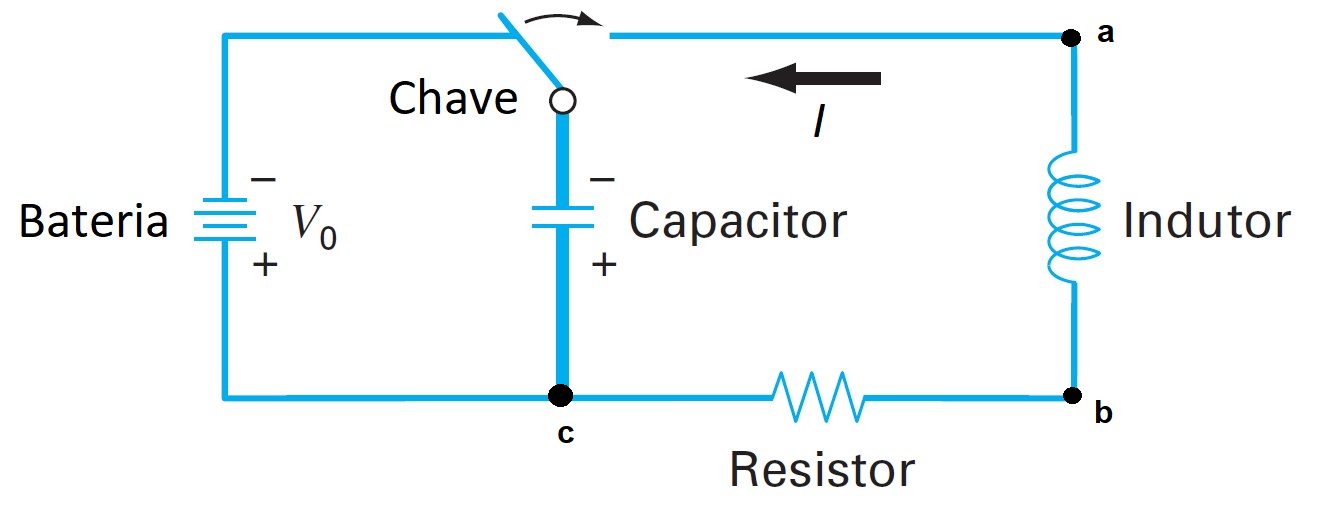
\includegraphics[height=5cm,width=12cm]{figura_1}%
\caption{Circuito RLC série a ser utilizado nas atividades do projeto}
\label{fig1}%
\end{center}
\end{figure}
O circuito apresentado na Fig. 1 é um circuito RLC, esse tipo de circuito apresenta uma carga cujo valor oscila com o tempo por existir uma resistência no circuito. Para estuda-lo, utilizamos a segunda lei de Kirchhoff, lei das malhas que é utilizada para encontrar as intensidades das correntes em circuitos elétricos, sendo aplicada aos caminhos fechados de um circuito, os quais são chamados de malhas. Os engenheiros elétricos geralmente a usam para estudar o comportamento estacionário de circuitos elétricos ou problemas que envolvem os circuitos que são transientes por natureza e em que ocorrem variações temporais súbitas, como o proposto no projeto. 

O que transcorre, é que quando a chave está aberta a bateria transfere a carga para o capacitor. Com o capacitor carregado, a chave seria fechada, com isso, cria uma corrente no circuito da resistência, do indutor e capacitor, até a carga do capacitor se esgotar, pois a resistência age como um dissipador de energia e depois de um certo tempo de ajuste alcança um novo estado estacionário. O objetivo desenvolvido no trabalho é encontrar qual o valor de resistência e indutância para cada uma das condições dadas, para isso, desenvolvemos um modelo físico e matemático e implementamos o modelo matemático para um programa afim de uma resoluçãao mais prática.\\

\textbf{Atividades de desenvolvimento:}\\
a)Determine uma expressão analítica para a variação da carga elétrica no circuito ao longo do tempo.\\
b)Determine o valor de R necessário para que o circuito dissipe a carga até atingir 1\% do seu valor original em t = 0,05 s, dado que L = 5 H e C = 0,0001F.\\
c)Determine o valor de L necessário para que o circuito dissipe a carga até atingir 1\% do seu valor original em t = 0,05 s, dado que R = 280 Ohms e C = 0,0001 F.

\section{MODELAGEM FíSICA}
O circuito a ser abortado no projeto é o mostrada na Fig. 1 e nele pode ser utilizada a segunda lei de kirchoff \cite{gussow2009eletricidade}. A segunda lei é a Lei de Kirchhoff para tensão, que afirma que a soma das tensões ao longo de um percurso fechado qualquer (malha) é igual à tensão total que está sendo fornecida a esse percurso , entao analisando o circuito separamos a malha da Fig. 2 para a analise das tensões \cite{dos2018caderno}.
% \ \ \ \
\newpage %
\subsection{Segunda lei de Kirchoff}
 Após serem analisadas as tensões podemos ver que temos uma tensão no resistor, uma no indutor e outra no capacitor, isto é

\begin{equation}
V_{ab}+V_{bc}+V_{ca}=0
\label{eq}
\end{equation}

Podemos escrever a Eq. (1) em termos das correntes e cargas em cada um dos elementos do circuito, como a seguir.

\begin{subequations}
\label{eqn:total}
\begin{equation}
\label{eqn:parcial}
L\frac{di}{dt}+Ri+\frac{q}{C}=0
\end{equation}

Sendo i = dq/dt, por definição de corrente elétrica, teremos:

\begin{equation}
L\frac{d^{2}q}{dt^{2}} +R\frac{dq}{dt}+\frac{q}{C}=0
\label{eqn:parcia1}
\end{equation}
\end{subequations}

A Eq. (2b) é uma equação diferencial de segunda ordem, completa e homogênea. 

\section{MODELAGEM MATEMÁTICA}
A equação diferencial de segunda ordem \cite{boyce2017elementary} Eq. (2b) foi resolvida utilizando a equação característica
\begin{equation*}
\alpha ^{2}+\frac{R}{L}\alpha +\frac{1}{LC}=0  .
\label{eq}
\end{equation*}
Após ser aplicada a fórmula de Bhaskara e terminando a resolução da equação diferencial de segunda ordem temos:
\begin{equation}
q(t)=C_{1}e^{at}cos(bt)+C_{2}e^{at}sin(bt)
\label{eq}
\end{equation}
Utilizando a Eq. (3) e aplicando as condições iniciais $C_{1}={q}(0) $, $ C_{2}={q}'(0) $ e $ {q}'(0)=i=0 $
obtemos que $C_{1}=q_{0}$  e  $ C_{2}=\frac{-aq_{0}}{b}$, obtendo assim que
\begin{equation}
\label{eq}
q(t)=q_{0}e^{at}cos(bt)-\frac{aq_{0}}{b}e^{at}sin(bt).
\end{equation}
Utilizando uma das informações dadas para a resolução do problema, 1\% do valor original da carga, temos que $q(t)=0.01q_{0}$ e utilizando essa informação na Eq. (4) temos as novas funções:
\begin{equation}
f(R)=e^{at}Cos(bt)-\frac{a}{b}e^{at}Sin(bt)-0.01\\ \textrm{onde:} \\a=-\frac{R}{2L}\\ \textrm{e} \\b=\sqrt{\frac{1}{LC}-\left ( \frac{R}{2L} \right )^{2}}
\label{eq}
\end{equation}
e
\begin{equation}
f(L)=e^{at}Cos(bt)-\frac{a}{b}e^{at}Sin(bt)-0.01\\ \textrm{onde:} \\a=-\frac{R}{2L}\\ \textrm{e} \\b=\sqrt{\frac{1}{LC}-\left ( \frac{R}{2L} \right )^{2}}
\label{eq}
\end{equation}

\section{MODELAGEM COMPUTACIONAL}
Utilizando Eq. (5) e Eq. (6) podemos então começar a resolver o problema aplicando um método númerico \cite{chapra2008metodos}.
Tendo em mente que a função dependendo dos valores dados será uma $f(R)$ ou uma $f(L)$, será utilizado o método da bisseção, que consiste em escolher um intervalo [a,b] que tenha a raiz da função nele e acharmos um valor aproximado da raiz. 

Para sabermos em qual intervalo há uma raiz será analisado o gráfico das funções e escolhido o melhor intervalo. Após serem plotados os gráficos de $f(R)$ e $f(L)$ foi notado que o gráfico de $f(L)$ (Fig.2) não passava pelo eixo $x$ logo, não seria possível achar o valor da raiz aproximada, mas o gráfico de $f(R)$ (Fig. 3) passava pelo eixo $x$ então foi utilizado o método da bisseção na função $f(R)$ e o valor obtido foi aproximado para o inteiro mais próximo e utilizado no valor de $R$ da função $f(L)$ chegando ao gráfico da Fig. 4.

Com os gráficos em mãos foi então utilizado o fluxograma da Fig. 5 para programar o método da bisseção na linguagem C++.

\begin{figure}[H] %h or !htbp
\vspace{-2pt}
\begin{center}
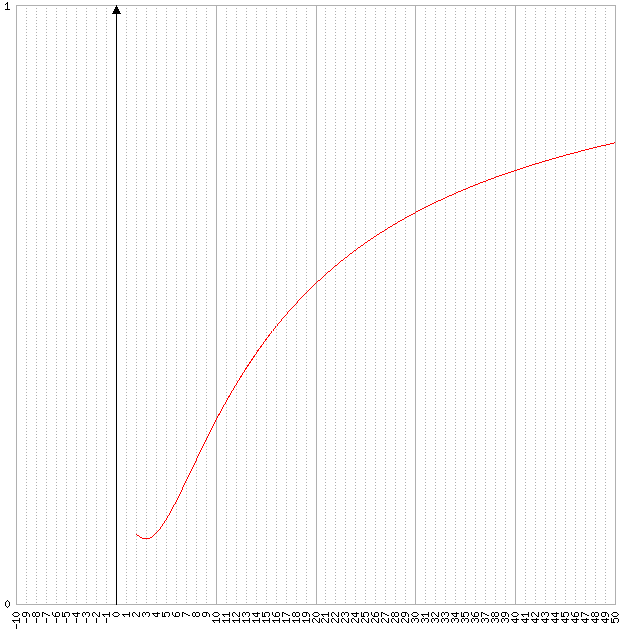
\includegraphics[height=10cm,width=10cm]{figura_5}%
\caption{Gráfico $f(R)$}
\label{fig4}%
\end{center}
\end{figure}

\begin{figure}[H] %h or !htbp
\vspace{-2pt}
\begin{center}
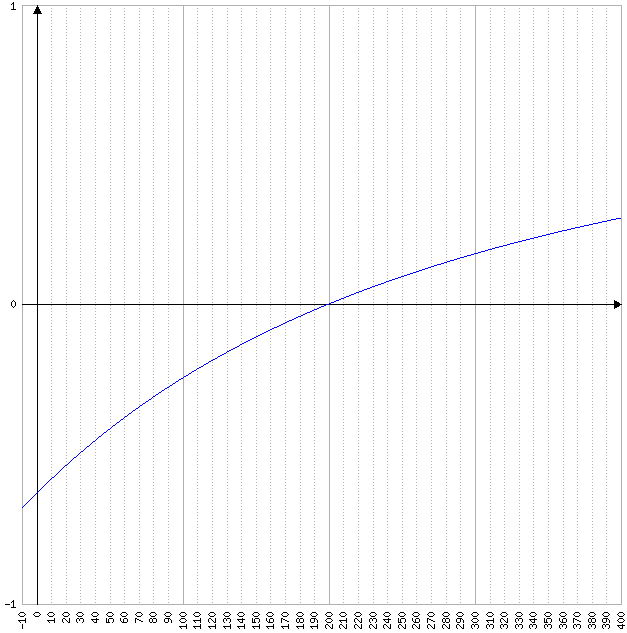
\includegraphics[height=10cm,width=10cm]{figura_4}%
\caption{Gráfico $f(L)$ com $R$=280}
\label{fig5}%
\end{center}
\end{figure}

\begin{figure}[H] %h or !htbp
\vspace{-2pt}
\begin{center}
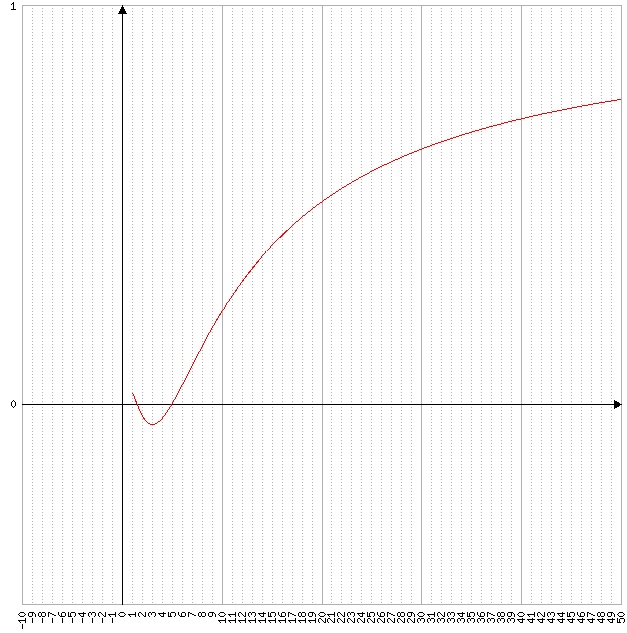
\includegraphics[height=10cm,width=10cm]{figura_6}%
\caption{Gráfico $f(L)$ com $R$=200}
\label{fig6}%
\end{center}
\end{figure}

\begin{figure}[H] %h or !htbp
\vspace{-2pt}
\begin{center}
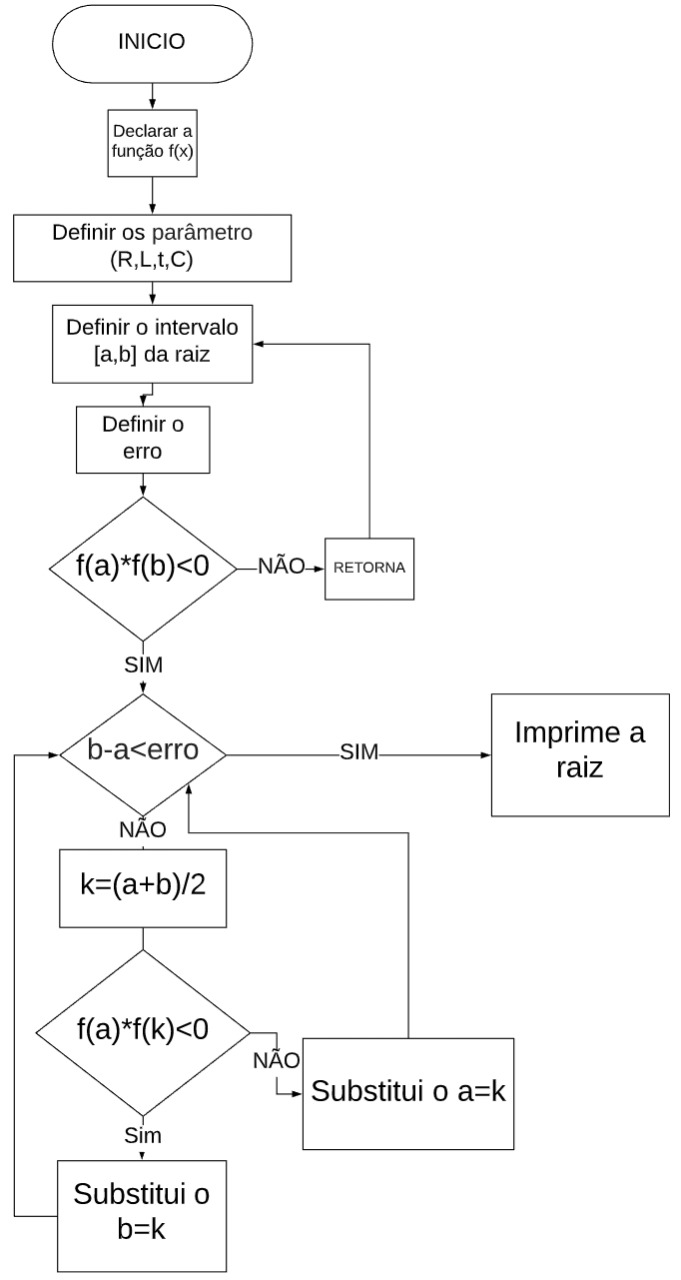
\includegraphics[height=18cm,width=12cm]{figura_3}%
\caption{Fluxograma para o programa em C++ que implementa o método da bisseção no problema}
\label{fig3}%
\end{center}
\end{figure}

\section{RESULTADOS}
Após a aplicação do método da bisseção foram calculados os valores aproximados de R para o item b e de L para o item c, os valores aproximados calculados pelo programa foram:\\ \\
b) R= 197,93 Ohms, com o intervalo [0,400].\\
c) L = 1,50 H, com o intervalo [1,4] e L = 4,9 H, com o intervalo [2,6].

\section{DISCUSSÃO}
O estudo do presente relatório inclue um circuito elétrico, composto por uma resistência (R), um indutor (L) e um capacitor (C), cujo circuito é chamado circuito RLC. Esse sistema também é abastecido por uma bateria separada por uma chave que carrega o capacitor na primeira posição. É apresentado o passo a passo da modelagem física, matemática e computacional do projeto, que tem por objetivo chegar ao valor da resistência para as condições L=5H, C=0.0001F, t=0.05s e carga igual a 1\% da carga inicial, e do indutor para as condições R=280 Ohms, C=0.0001F, t=0.05s e carga igual a 1\% da carga inicial. Para alcançar tal objetivo, foi necessário recorrer à Lei de Kirchhoff para tensões. Portanto, chegando a uma EDO ao passo que aplicou-se um método matemático para encontrarmos a solução numérica do problema, que será apresentada ao final deste relatório.

% ------------------------------------------------------------------------
\bibliographystyle{plain}
\bibliography{modcomp}
\vspace*{-0.1cm}
% ------------------------------------------------------------------------

\end{document}
